\chapter{Manual de utilização} \label{manual}

Para usar o sistema desenvolvido, terá de executar os seguintes passos dentro da pasta Install:

\begin{enumerate}
	\item Lançar o executável \textit{CentralManagerServer.exe} que consta dentro da pasta Central Manager;
	\item Dentro da pasta Brokers, existem duas pastas. Em cada uma delas, deverá lançar o executável \textit{BrokerServer.exe};
	\item Para executar um ou mais clientes, deverá lançar o executável \textit{UserFormImpl.exe} presente na pasta User, consoante o número de utilizadores desejado.
\end{enumerate}

\section{Utilização do Cliente}

\begin{figure}[h]
	\makebox[\textwidth][c]{
		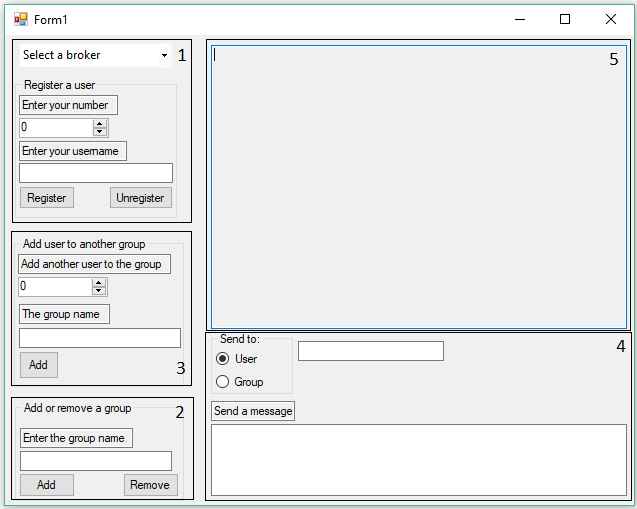
\includegraphics[width=0.9\textwidth]{./figures/form}
	}
	\caption{User Form}
	\label{form}
\end{figure}

Na figura \ref{form} é apresentada a interface gráfica do utilizador.
Relativamente a esta figura, existem retângulos numerados. Cada retângulo é explicado de seguida.\\

No retângulo 1, pode selecionar o \textit{broker} à qual o utilizador pretende-se registar. Para tal, necessita de indicar o seu número e o seu nome. Para se registar, deve preencher o formulário e carregar no botão \textit{Register}. Para fazer \textit{Unregister}, deve carregar no botão \textit{Unregister}.\\

No retângulo 2, existe a possibilidade de criar ou remover grupos. Para criar ou remover um grupo, basta indicar o seu nome e carregar no botão \textit{Add} ou \textit{Remove} para adicionar ou remover um grupo, respetivamente.\\

No retângulo 3, pode adicionar um utilizador a um dado grupo à qual pertence. Para realizar esta operação, deverá indicar o número do utilizador que pretende adicionar e o nome do grupo ao qual irá adicionar. Havendo preenchido o formulário, deverá carregar no botão \textit{Add}.\\

O retângulo 4, permite enviar mensagens para um utilizador ou para um grupo. Para enviar uma mensagem para um utilizador, deverá selecionar o \textit{radio button User} e indicar o número do utilizador à qual pretende enviar a mensagem. A caixa de texto \textit{Send a message} permite escrever a mensagem que pretende enviar. Para enviar, basta pressionar o botão do teclado \textit{Enter}. Se pretender enviar a mensagem para um grupo, o procedimento repete-se, diferindo apenas na escolha do \textit{radio button}, que deverá ser \textit{Group}.\\

O retângulo 5 é onde se apresenta as mensagens enviadas e recebidas, quer por utilizadores, quer por grupos. As mensagens vêm identificadas pelo nome do utilizador caso exista. Caso contrário, são identificadas pelo número do utilizador. 